\documentclass[11pt]{article}

\usepackage[T1]{fontenc}
\usepackage[margin=1in]{geometry}
\usepackage{graphicx}
\usepackage{hyperref}

\setlength{\parindent}{0pt}
\setlength{\parskip}{0.5em}

\title{Pulp Governance}
\author{Pedro Brochado}
\date{\today}

\begin{document}

\maketitle

\begin{abstract}
  Summarize the governance question, the proposed approach, and the intended
  outcome. Replace this note when the central argument is clear.
\end{abstract}

% -------------------------------------------------------------------------------
\section{Revision}
\begin{itemize}
  \item \emph{Red Hat's CRA position}: industry context on lifecycle security \cite{redhat-cra}.
  \item \emph{Stewardship guidance}: Red Hat's stated role and practices for Pulp \cite{redhat-cra-steward}.
  \item \emph{Community health audit (2018)}: historical governance and process context \cite{pulp-health-audit}.
  \item \emph{The Open Source Way}: governance roles, policies, and community evolution \cite{open-source-way-governance}.
  \item \emph{Pulp governance repository}: current project policies and processes \cite{pulp-governance-repo}.
\end{itemize}

Document the existing governance arrangements and cite primary sources for
claims about current roles, processes, or policies. For an industry perspective
on CRA readiness and open-source software stewardship, see \cite{redhat-cra,
redhat-cra-steward}. For historical community-health and governance context,
see the Pulp Community Health Audit Report \cite{pulp-health-audit}.


% -------------------------------------------------------------------------------
\section{Opening screen}

Hello everyone, this presentation is about the new governance repository in the Pulp Project.

\subsection{Roadmap}
We'll start with a general introduction to governance, the we'll jump into what's new with
that repository and finally throw some ideas for the future.

\subsection{Self-Presentation}
First let me introduce myself:
My name is Pedro, I'm a software engineer at Red Hat since 2023,
I work full time at the Pulp Project.
and I have 2 cats that manages my remote work very closely.
% TODO: photo wiht Red Hat hat, pulp jacket and my cats on my PC.

\subsection{Disclaimer}
Before I start, I just wanna give a disclaimer.

I've been a software engineer for a living for not this long time, but from the start,
and even before the start really, I was driven to the world of open source.
The reason is that \textbf{I really do believe} that some of the principles associated with open-source,
like collaboration, transparency and freedom, are really important in any human activity.

Despite that, I must confess I've never really dived deep into the topic of governance in open-source,
which was a mistake, because after I started thinking and researching more about it, I started to realize and appreciate
how vital it is the role governance in making these principles effective in practice.

So the disclaimer here is that I won't present you with in-depths concepts and authoritaive information
- simply because I don't have them.
My humble goal is to share some of my recent enthusiams for the topic, and I hope you find that inspiring
or useful!

% -------------------------------------------------------------------------------
\section{Open-Source and Governance}
% Define what governance is and why it matters.
% Present governance models by example (community/forgeo, company/nextjs, foundation/k8s)
% Try to situate Pulp as company-baked with an openess for extensions (e.g, outside collaborators)

\subsection{Introduction}
So let's get started.

In this section I want to show just a few examples governance in open-source projects.
First things first:

\subsection{What is governance?}
% Define what governance is and why it matters.

According to this great website, theopensourceway.org, it can have different meaning in different contexts.
I like one of the quotes which is very incisive, which says that governance:

\begin{quote}
(...) a system of \textbf{rules, roles, and procedures} that determine how \textbf{power}
in an organization gets distributed.
\end{quote}
% TODO: cite the opensourceway.org

The open-ended part of this definiton is: who is part of an open-source project organization?

My personal temptative answer is that developers, the users and possibly the companies behind them
are all part of that organization, whether that is explicitly stated or not.

They all have different interests which are possilby conflicting,
and the first thing a governance does is making that power distribution transparent.
It's showing who, how and when one can influence a project's direction.

So now let's see a few governance models, and how they distribute that power.

\subsection{Governance models}
First, these are just some examples.
The mix of models depends on what a project goal is, how big is it and various other factors
I cannot discuss here.
\cite{open-source-way-governance}.

\subsubsection{Do-ocracy}
So let's see the do-ocracy model.
This tends to fit smaller, informal projects:
the people doing the work make the decisions, and influence grows through
contributions.

The more you participate, the more trust and power you gain.

\subsubsection{Founder-leader}
Then there's the founder-leader model, where the founder has the final say.
and Python is probably the canonical example of this.
Guido van Rossum was the founder-leader for a lot of years, but
he stepped down in 2018, and the project moved to an elected steering council

The degree in which other members can influence decisions has to do with how benevolent
the founder-leader is, so you might also have heard of the role of a founder-leader as
BDFL, or ``benevolent dictator for life.'' 
\cite{python-governance}.

\subsubsection{Electoral}
Then there is the electoral model. People with voting rights choose the
project's leaders, and sometimes decide on important policies too.

Debian is a good example. Its developers elect the project leader every year,
and they can also vote on general resolutions \cite{debian-constitution}.

This model distributes power more evenly, and it is usually very well structured,
but requires a good deal of organization and active community members.

\subsubsection{Single-vendor}
This is the case where there is one company behind the project development.
Next.js, for example: Vercel's core team explicitly leads the project, even though people
outside Vercel contribute too \cite{nextjs-governance}.

The amount of openess can vary greatly, but ultimetly company-baked team has the final call.

\subsubsection{Foundation-backed}
And finally, there's the foundation-backed model. A foundation helps look after
the project's resources and support its community.

The Cloud Native Computing Foundation (CNCF) is a great example.
The foundation is behind a lot of project, which contains different levels of compliance
to a very well defined set of project standards.

For example, it has mechanism to ensure a project has a diversity of members from different
companies, so no single-vendor dictates de direction of the project.

It also establishes that projects under the organization has some specific \textbf{governance artifacts},
like a MAINTAINERS.md file, which codifies ownership and brings transparency on the project roles.

This is great for projects that need robust strategies, standards and protocols,
which beneft a lot from diversity and cooperation among bigger stakeholders.
Some examples are Kubernetes and Linux. \cite{cncf-kubernetes}

\subsubsection{And Pulp?}

And Pulp, what is Pulp's model?

This was the core question that motivated me to create the pulp/governance repository.

I think the most straighfoward observation we can make is that the project is baked by Red Hat,
which matches the singler-vendor definition, which should be not a surprise not anyone.

But there is not only that. We have Red Hat as the main company behind it, but we also have other companies
directly involved in plugin and core development, we have companies that uses Pulp in a lot of important places
and we even have individuals that just wanna make contributions of their own!

And we have to look into all of this.

So this is an invitation for us to think about answering that question.

Putting that in more appealing words:

\begin{quote}
How can we - members of the Pulp community - understand and shape our governance to maximize the value of this piece of software,
which plays such as crucial role in todays industry?
\end{quote}

\subsubsection{Recap}

Quick recap:

We've seen governance as a set of rules, roles and produces that determine distribution of power;
We've seen 5 example models of how can a project shape it's governance;
And finally we were provoked to think about how good governance can help a project leverage
the full power of it's community and of it's open-source nature.

% -------------------------------------------------------------------------------
\section{Governance in Pulp}

Great, we concluded the first half of the talk!

Now let's see more closely of what this pulp is made of.
% TODO picture of zoom of a citrus fruit

\subsection{Rules, Roles and Prodecures}
% High-level of governance in Pulp, existing documents and processes:
%   standard "community health files": CoC, Privacy, Security, Contribution
% Work and discussion on AI policies
%   New artifact: AI Policy - a lot of discussion around it
Here, I'll briefly describe some of the constituints of how the project operates.
I'll probably leave something behind, so please forgivem ahead of time.

\subsubsection{Rules}
The project has most of the basic artifacts expected from an open-source projects, and which
can be used as metrics of a project health.
These includes Code Of Conduct, Privacy Notice, License files, Contributing and more recently an AI Policy.

Without getting into too much details, I believe these \textbf{governance artifacts} does
a decent job a defining the general rules and principles behind the project.

It's worth calling out the AI Policy, which is one which had a lot of attention lately.
As other projects, the Pulp project has received a fair amount of low quality AI PRs and reports,
and we tried (and are actively trying) to design this policy as to reduce the maintainace burden
of these while allowing responsible and accountable use of the AI as a tool. \cite{pulp-ai-policy}

But in what concerns pulp/governance repository, the idea is that it becomes the authoritative source
of truth for all \textbf{governance artifacts}.

\begin{center}
  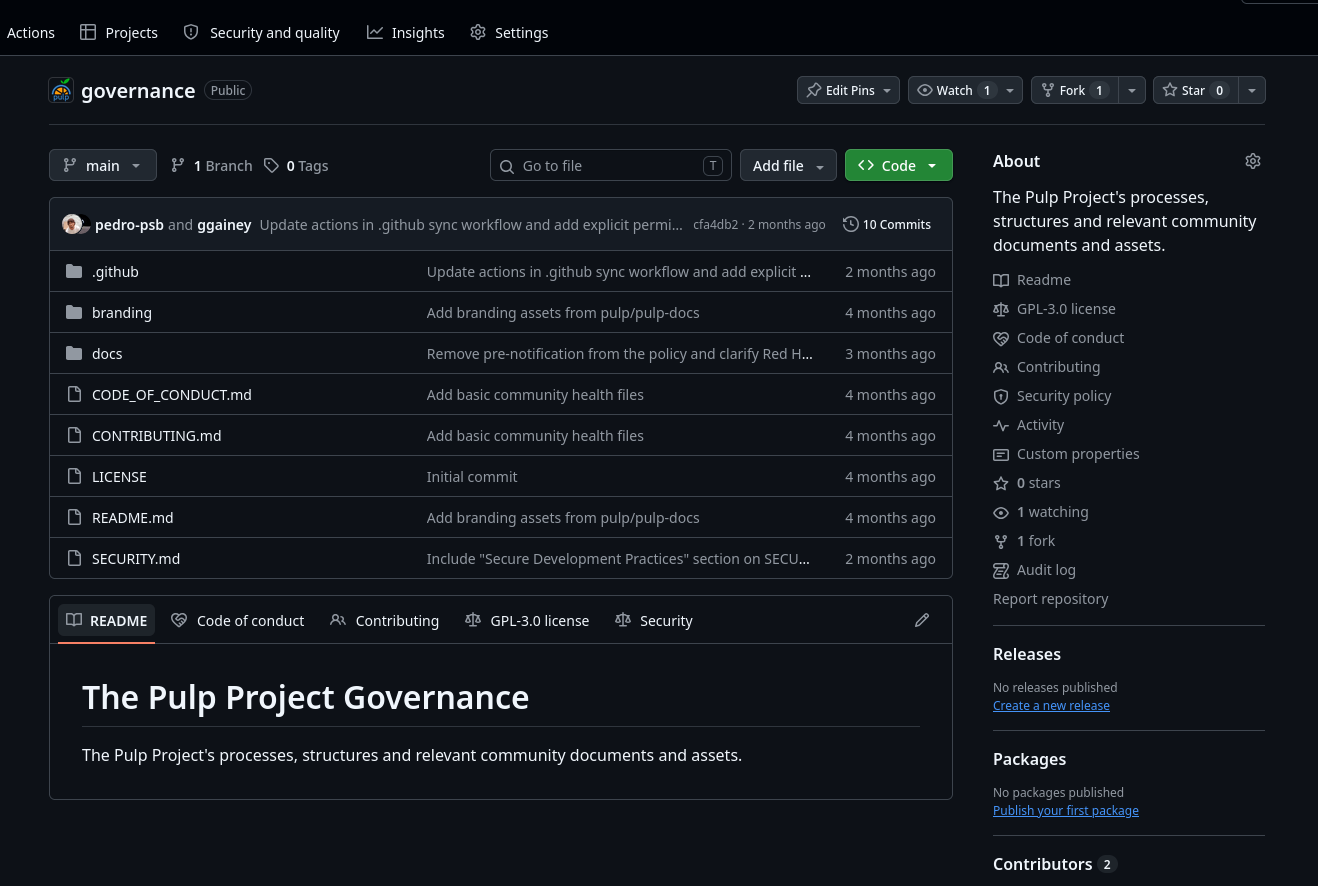
\includegraphics[width=\linewidth]{images/pulp-governance-repository.png}
\end{center}

\begin{minipage}{\linewidth}
This idea was directly inspired by forgejo governance repository:

\begin{center}
  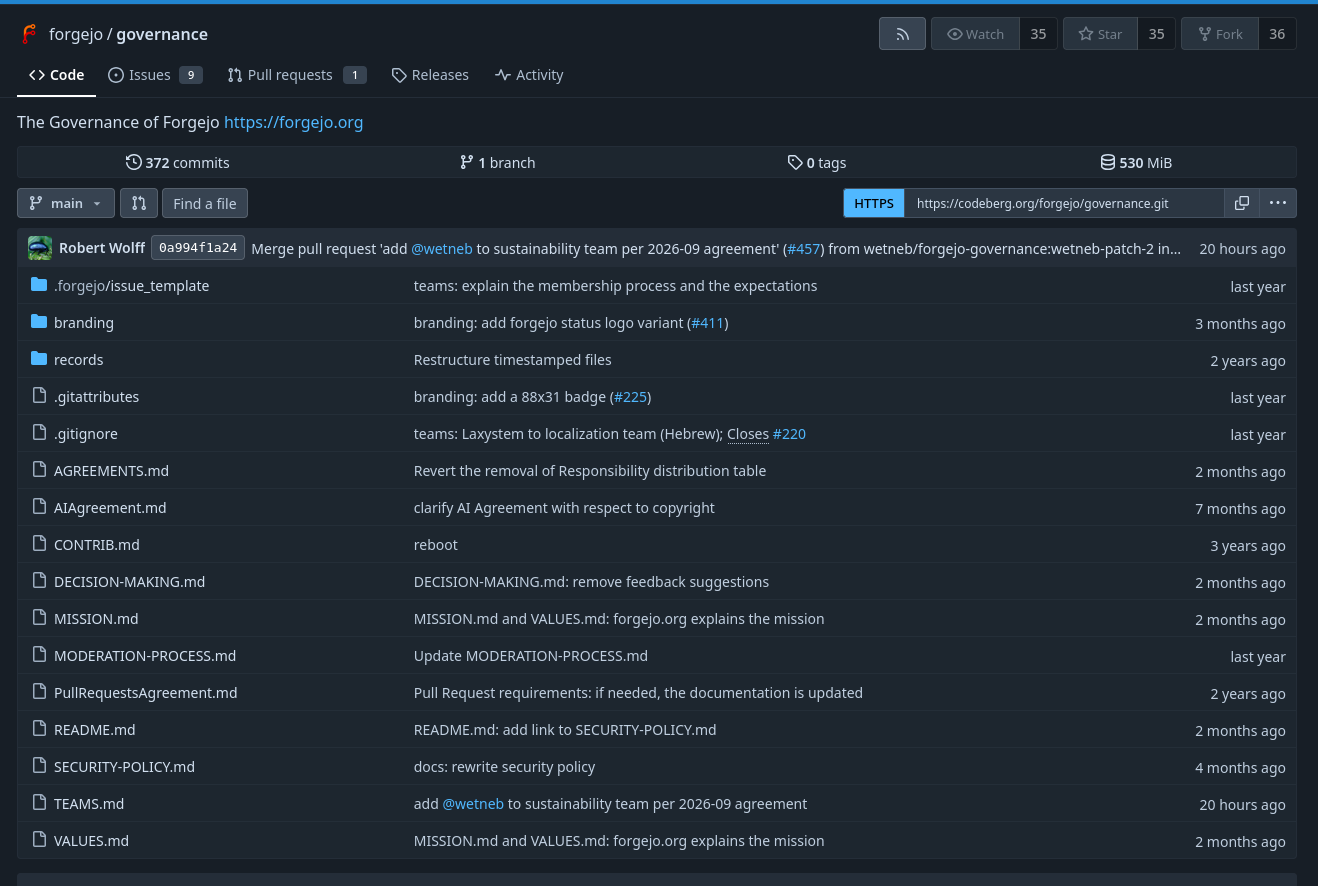
\includegraphics[width=\linewidth]{images/forgejo-governance-repository.png}
\end{center}
\end{minipage}

\subsubsection{Roles}

I'll start that with a critique, which is that
the project does not have a formal definition of roles which anyone can look an understand.
But I'll say more about that in the next section.

In any case, the project does have implicit and event explicit roles.

The existing explicit roles are github teams and roles, which we do use to a certain degree
to encode permissions and responsabilities.

But there are also conceptual implicit roles we don't encode, such as
redhatters and non-redhatter maintainers, which does have different levels of power;
the concept of plugin leaders, and more recently we have informally introduced a Benevolent Dicator...
ah, I mean, a tech lead role, which is Grant.

I'm really kidding, it's not a Benevolent Dicator for Life, sorry Grant.

We felt the need for this new role to help untie more challening proposals which have grater
technical and political impact with more agility.

\subsubsection{Procedures}

We do have some documented and some undocumented processes.
As fair as I know, the most important ones are documented, such as:
the community integration meetings with katello, where the core team collaborates with katello
folks from Red Hat and from Atix, which is another company that uses Pulp/Katello;
We have weekly open pulpcore meetings and open-floor meetings, where anyone can put topics, join
and discuss;
We also have weekly bug triage, which is a in-chat meeting where go through untriaged items to
either accept or decline requests.

We also have release rotation, meeting lead rotation, discourse sheparding, and a lot of other
more internal processes I won't go in depth here.

\subsection{EU Cyber Resilient Act}
% The creation of pulp/governance and CRA work
%   Pitch how these were independent, but one heped the other
%   Explain what CRA is, what is

\subsection{Opportunities}
% Process project health audits
%   show the audit from Brian and Ina
%   give examples of how we always are trying to keep up with this
% Structured and clearer roles:
%   Show the case of CNFC with MAINTAINERS.md files (automatable)
%   Share idea about a "formal" user role, where the user/company that uses pulp
%   publicily "registers" itself as a "project user" (giving rights for pulp to share their naems),
%   and privately share their contact information for important communications and informations
%   (e.g, plugin will be discontinued by core maintainer, a breaking change, etc...)
% Automated audits (briefly):
%   Show the UK tool for automated audits. 

% -------------------------------------------------------------------------------
\section{Closing words}
% \begin{quote}
At its heart, open source project and community governance is about people - their
\textbf{rights and responsibilities} as part of a project and \textbf{the expectations others have for them}.
% \end{quote}


% -------------------------------------------------------------------------------
\section{References}
\begin{thebibliography}{99}
  \bibitem{redhat-cra}
  Red Hat. \emph{Red Hat and the EU Cyber Resilience Act (CRA)}.
  Updated March 4, 2026. Accessed November 6, 2026.
  \url{https://www.redhat.com/en/red-hat-eu-cyber-resilience-act}.
  Local source note: \path{references/red-hat-eu-cyber-resilience-act.md}.

  \bibitem{redhat-cra-steward}
  Red Hat. \emph{EU Cyber Resilience Act Stewardship Guidelines for Red Hat
  Supported Open Source Projects}. Updated June 12, 2026. Accessed November 6,
  2026. \url{https://access.redhat.com/security/eu-cyber-resilience-act-stewardship-guidelines}.
  Local source note:
  \path{references/red-hat-eu-cyber-resilience-act-stewardship-guidelines.md}.

  \bibitem{pulp-health-audit}
  Pulp Project. \emph{Pulp Community Health Audit Report}. September 17, 2018.
  Accessed November 6, 2026.
  \url{https://pulpproject.org/blog/2018/09/17/pulp-community-health-audit-report/}.

  \bibitem{open-source-way-governance}
  The Open Source Way contributors. \emph{Project and Community Governance}.
  Accessed November 6, 2026. Licensed under CC BY-SA 4.0.
  \url{https://guidebook.theopensourceway.org/growing-contributors/project-and-community-governance}.
  Local Markdown copy: \path{references/the-open-source-way-project-and-community-governance.md}.

  \bibitem{python-governance}
  Python Project. \emph{PEP 13: Python Language Governance}.
  \url{https://peps.python.org/pep-0013/}.

  \bibitem{node-governance}
  Node.js. \emph{Project Governance}.
  \url{https://nodejs.org/en/about/governance/}.

  \bibitem{debian-constitution}
  Debian Project. \emph{Debian Constitution}.
  \url{https://www.debian.org/devel/constitution}.

  \bibitem{nextjs-governance}
  Next.js. \emph{Governance}.
  \url{https://nextjs.org/governance}.

  \bibitem{cncf-kubernetes}
  Cloud Native Computing Foundation. \emph{Kubernetes}.
  \url{https://www.cncf.io/projects/kubernetes/}.

  \bibitem{pulp-governance-repo}
  Pulp Project. \emph{Pulp governance repository}. Accessed November 6, 2026.
  \url{https://github.com/pulp/governance/}.

  \bibitem{pulp-ai-policy}
  Pulp Project. \emph{AI Policy}.
  \url{https://github.com/pulp/pulp-docs/blob/main/pulpproject.org/help/more/governance/ai_policy.md}.
\end{thebibliography}

\end{document}
